% !TeX root = documentation.tex
% !TeX spellcheck = de_DE


\section{Lorenz-Modell}
Die Gleichungen, welche das Lorenz-Modell beschreiben, enthalten viele physikalische Eigenschaften wie die Dichte, Geschwindigkeit und Temperatur der Atmosphäre und stellen diese physikalischen Werte formalisiert dar. Lorenz wollte aus den bereits existierenden Gleichungen der Hydrodynamik ein Modell zur Wetterprognose erstellen. Basierend auf vorgehenden Werken von Saltzman startete Lorenz mit den hyrodynamischen Gleichungen und verfolgte ein systematisches Näherungsvorgehen, womit er auf die folgenden drei Gleichungen stoss:

\begin{align}
\dot{x} &= \sigma(x - y)\\
\dot{y} &= x(\rho - z) - y\\
\dot{z} &= xy - \beta z
\end{align}

Die X-Achse entspricht dabei der hydrodynamischen, räumlichen Durchschnittsgeschwindigkeit, also die durschnittliche Windgeschwindigkeit. Die Y-Achse repräsentiert die Temperatur und die Z-Achse der Temperaturgradient. Also wie schnell sich die Temperatur verändert. 

Wie aus den obigen Gleichungen ersichtlich ist, sind drei Parameter vorhanden. Alle sind immer positiv.

\subsubsection{1. Parameter: $\sigma$}
$\sigma$ entspricht der dimensionslosen Prandtl Nummer. Diese ist das Verhältnis von \textit{Viskosität} und der \textit{Währmeleitfähigkeit}. Da beide Eigenschaften die Einheit $\frac{m^2}{s}$ haben, resultiert daraus eine dimensionslose Zahl.

\subsubsection{2. Parameter: $\rho$}
Dieser Parameter ist nach dem Physiker Baron Rayleigh benannt worden und heisst Rayleigh Zahl. Es entspricht dem Verhältnis von \textit{Wärmeausdehnung} und der \textit{Viskosität}.

\subsubsection{3. Parameter: $\beta$}
Der dritte Parameter des Lorenz-Modells ist das $\beta$. Es entspricht der Wärmeausdehnung. Dabei handelt es sich um die Veränderung der geometrischen Grössen eines Körpers, die sich mit erhöhter Temperatur vergrössern. Dehnt sich ein Körper aufgrund der Temperaturänderung aus, so verändert sich auch stets die Dichte.

\begin{figure}
	\centering
	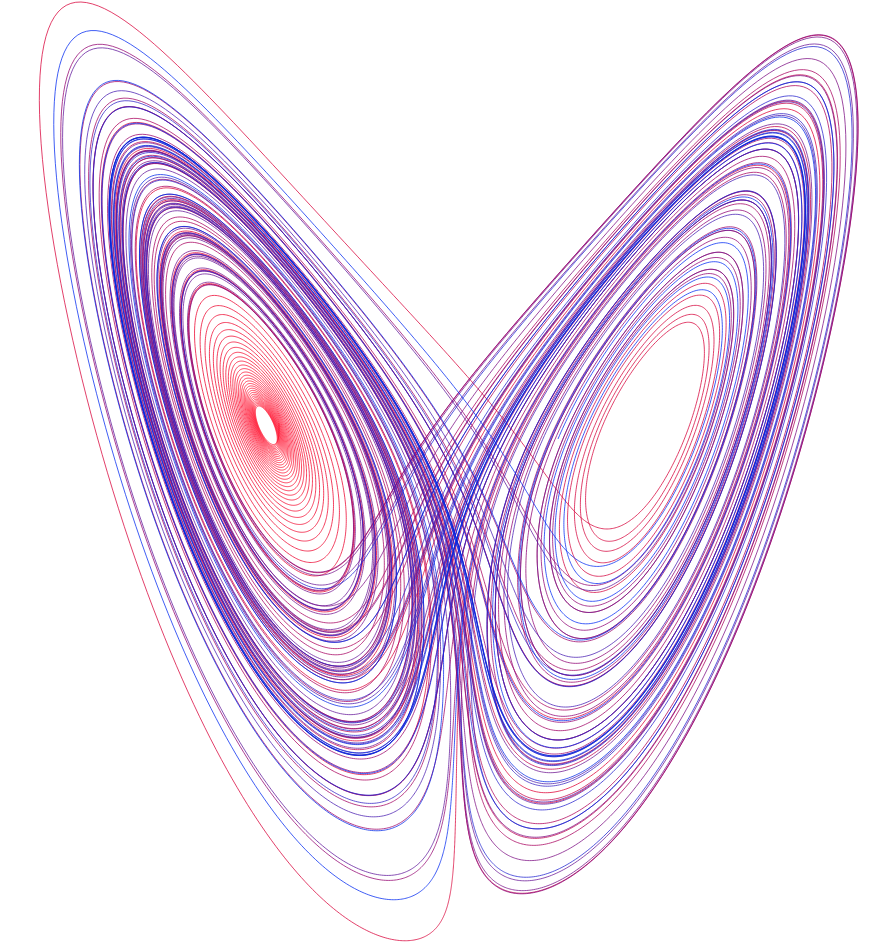
\includegraphics[width=0.3\linewidth]{lorenz/assets/lorenz-modell/lorenz-modell}
	\caption{Lorenz-Modell}
	\label{fig:lorenz-modell}
\end{figure}


\subsection{Eulersches Verfahren}
Es gibt für das Lösen von Differentialgleichungen zwei Ansätze. Zum einen der analytische Ansatz, der eine allgmeingültige Lösung sucht. Es handelt sich bei den drei Lorenz-Gleichungen um nicht-lineare Differentialgleichungen, welche analytisch nicht lösbar sind. Aus diesem Grund fällt dieser Ansatz weg. 

Der zweite Ansatz ist, eine Diskretisierung vorzunehmen und den Computer für jeden definierten Zeitpunkt die Resultate der Gleichungen ausrechnen zu lassen. Dies ist auch der in dieser Arbeit gewählte Ansatz, der im Folgenden bis zur tatsächlichen Visualisierung genauer beschrieben wird. 

%TODO Betitlung
\subsubsection{Eulersches Verfahren}

Das Ziel vom eulerischen Näherungsverfahren ist es hier, die Differentialgleichungen approximativ zu lösen. Durch eine Diskretisierung der Werte können wir eine Form der Gleichungen bestimmen, die später visualisiert werden können. Um die Ableitung zu berücksichtigen, muss das Ergebnis einer Differenzialgleichung zu einem diskreten Zeitpunkt für die Berechnung des nächsten Zeitpunktes addiert werden. So wird die Steigung an einem Punkt t berechnet. Diese Steigung können wir in eine lineare Gleichung einsetzen und daraus den absoluten Punkt berechnen.

Der \textit{Y-Achsenabschnitt} wird mit dem Ergebnis der vorherigen Rechnungsschritt belegt, da der Differenzalterm den Abstand vom Wert vorher berechnet.  

\begin{align}
\label{LGResult}
% TODO: Lorenzgleichung umschreiben
y(t + 1) &= \frac{d LG}{d t} \cdot  \Delta t + y(t) & LG = Lorenzgleichung
\end{align}

Dieses Verfahren kann auf alle Koordinaten des Lorenz-Systems angewendet werden.

Eingefügt in die Gleichung \eqref{LGResult} ergibt sich folgendes System:

\begin{align}
x(t+\Delta t) = x(t) + \frac{dx}{dt} \cdot \Delta t\\
y(t + \Delta t) = y(t) + \frac{dy}{dt} \cdot \Delta t\\
z(t + \Delta t) = z(t) + \frac{dz}{dt} \cdot \Delta t
\end{align}

Das angewendete Verfahren nennt sich \textit{Eulersches-} oder \textit{Einschritt-Verfahren}. Durch das, dass wir einen numerischen Ansatz mit dem Euler Verfahren gewählt haben, resultiert eine Annäherung des Lorenz-Attraktors. Da solche Abweichungen von der tatsächlichen Lösung existieren, ist zu erwarten, dass diese Abweichungen gross genug sind, um zum chaotischen Verhalten beizutragen. Es gäbe auch genauere Verfahren für das numerische Lösen der Gleichungen wie das \textit{Quadratische Verfahren} oder das \textit{Runge-Kutta Verfahren}. Da aber auch bei diesen Verfahren keine absolute Genauigkeit erreicht wird, blieben wir bei der Eulerschen Annäherung. 
